\documentclass[12pt,a4paper,oneside,brazil]{abntex2}

% Pacotes que serão utilizados%
\usepackage{lmodern}
\usepackage[utf8]{inputenc}
\usepackage[brazil]{babel}
\usepackage[T1]{fontenc}
\usepackage{indentfirst}
\usepackage{graphicx}
\usepackage{microtype}
\usepackage{amsmath}
\usepackage[backend = biber, style=abnt]{biblatex}
\addbibresource{Referencias.bib}

% Informações do documento %
\title{Notas Economia Matemática}
\author{Thiago Oliveira Coelho}
\date{\today}



\begin{document}
\pagestyle{plain}
\pagenumbering{arabic}

\maketitle

A matemática cada vez mais se torna a linguagem da economia, ela nos ajuda a explicitar melhor e remover as dualidades das proposições teóricas. Um modelo matemático tem de ser enunciado de modo claro e prático, com isso pode ser mais facilmente criticado e modificado. Como exemplo podemos tomar a escolha entre bens do agente microeconômico, que ordena suas preferências por cestas de modo que:
\[ U_3 \succ U_2 \succ U_1 \]
A cesta 3 concede mais utilidade ao agente que a cesta dois, que por sua vez é melhor que a cesta 3. O problema de composição desta cesta pode ser dado de modo:
\[ Max U = U( X_1, X_2, ..., X_n); P_1 X_1 + P_2 X_2 + ... + P_n X_n \leq M \]
O agente tenta maximizar sua utilidade compondo sua cesta com os bens X, mas a compõe tendo a restrição orçamentária M, ou seja, o preço de cada bem vezes a quantidade deste é somada a quantidade dos outros bens vezes o preço de cada um e esta soma tem de ser menor ou igual a M. A matemática simplifica em muito o processo de explicar este tipo de análise microeconômica, que se feita de modo puramente por meio de texto, pode ser extremamente confuso para o leitor. \newline
Este resumo é baseado em: \cite{chiang1984}, \cite{simon}, \cite{nicholson}, \cite{boldrini} e \cite{stewart}.
\clearpage

\tableofcontents

\chapter{Cálculo a uma variável}

\section{Reta numérica}
A matemática tem como sua base fundamental os números e as funções, para melhor representá-los utilizamos da análise gráfica e da geometria. Para esta análise geométrica precisamos da \emph{reta numérica}, uma linha que se estende indefinidamente para a direita e esquerda e que possui origem no número 0. Cada número Real é representado por exatamente um ponto na reta, sendo que números a direita da reta são positivos, e números a sua esquerda são negativos.

\section{Funções}
\section{Fundamentos}

Uma função é uma regra que associa um número em R a um outro número real, por exemplo, se quiser relacionar um número real qualquer ao seu dobro podemos utilizar:
\[ y = f(x) \rightarrow f(x) = 2x \]
Y é o uma função de X, sendo que esta função retorna uma valor que é duas vezes o valor inicial. Denominamos X de variável exógena ou independente e Y de variável endógena ou dependente. As funções podem ser mais simples, possuindo somente monômios, que aparecem da seguinte forma:
\[ f(x) = a x^k \]
Sendo $k$ o \emph{grau} do monômio e $a$ o \emph{coeficiente}. Funções mais complexas são compostas por polinômios, que são formados a partir da adição de polinômios:
\[ f(x) = a_1 x_1^{k_1} + a_2 x_2^{k_2} \]

Funções podem ser crescentes ou decrescentes:
\begin{enumerate}
\item Crescente: $ x_1 > x_2 \Rightarrow f(x_1) > f(x_2)$;
\item Decrescente: $ x_1 < x_2 \Rightarrow f(x_1) < f(x_2)$.
\end{enumerate}

Os pontos aonde uma função passa de crescente para decrescente ou vice versa configuram máximos ou mínimos. Se em nenhum outro momento a função passa deste máximo ou mínimo, este é um \emph{máximo ou mínimo global}. Toda função possui também um domínio, que é o conjunto de números que x pode assumir para os quais $f(x)$ existe e uma imagem, que é o conjunto de números que $f(x)$ pode assumir para os diversos valores de x.

\begin{figure}[ht]
\centering
    \begin{minipage}{0.45\textwidth}
        \centering
        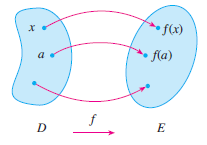
\includegraphics[width=0.75\textwidth]{Dominio.PNG}
        \caption{\cite[p. 11]{stewart}}
     \end{minipage}\hfill
     \begin{minipage}{0.45\textwidth}
        \centering
        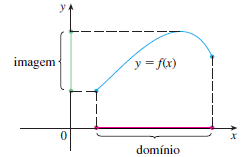
\includegraphics[width=0.75\textwidth]{Dominio2.PNG}
        \caption{\cite[p. 11]{stewart}}
    \end{minipage}
\end{figure}

\section{Função linear}
São polinômios de grau 1:
\[ f(x) = m x + b \]
Seu gráfico será caracterizado por uma linha reta. Sua inclinação será o quociente da mudança entre coordenadas e medirá a taxa de variação da função:
\[ \frac{y_1 - y_0}{x_1 -x_0} \]
Como a relação é linear, a inclinação será sempre a mesma para qualquer ponto da reta.


\section{Funções não lineares}
Para obtermos a inclinação de tal função em certo ponto $P$, podemos desenhar uma tangente (reta que toca a curva neste ponto e possui mesma direção) deste forma:

\begin{figure}[ht]
\centering
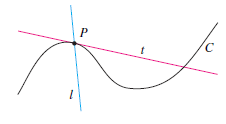
\includegraphics[scale=0.8]{Tangente.png}
\caption{\cite[p. 76]{stewart}}
\end{figure}

A inclinação da reta tangente neste ponto P é igual a derivada da
função naquele ponto. Essa reta tangente é encontrada ao desenharmos 
várias retas secantes (que cortam o gráfico mais de uma vez) a partir
 de tal ponto, avançando na função sempre o mínimo possível. Essa inclinação num ponto de coordenadas $ 
 (A, f(A) $, sendo $h_n$ uma sequência de números tão pequenos que chegam a tender monotonicamente
 a zero:

\begin{equation}\label{inclinação tangente}
f'(X) = \lim_{h \rightarrow 0} \frac{f (X_0 + h) - f (X_0)}{h}
\end{equation}

Essa  reta secante é uma boa aproximação da tangente, e consequentemente da inclinação da função naquele ponto.


A inclinação da reta tangente no ponto $X_0$ é a \emph{derivada} da função em $X_0$

\subsection{Diferenciabilidade e Continuidade}
Um função é derivável se puder ser derivável em todo ponto de seu domínio. Isso significa que em geral somente funções com gráficos de 'curvas suaves' são diferenciáveis em cada ponto. Já uma função continua leva a seguinte definição: \newline

Uma função $ f: D \rightarrow R^1$ é contínua num ponto x se dada sequência ${X_n}$ que converge a x em D, $ f (X_n)$ converge a $ f (x)$. \newline

Em geral as funções contínuas apresentam gráficos sem rupturas. Uma função cuja reta tangente obtida pela derivada em um ponto $(x, f (x)$ varia continuamente com x é chamada de \emph{Continuamente diferenciável} ou \textbf{$C^1$}. Se a segunda derivada da função varia com x então a função é dias vezes continuamente diferenciável ou \textbf{$C^2$}. Em geral assumimos que as funções econômicas são contínuas se não diferenciáveis. Se temos uma função de produção do estilo: $y = f (x)$, é razoável supor que uma mudança marginal na quantidade de insumo provoca uma mudança na quantidade produzida. Para computarmos exatamente esta mudança, lembre que numa função linear $ y = m x + b$ m é a inclinação e portanto explica todo o impacto de uma variação em b: $\triangle y = \triangle x$. Para funções não lineares, se utilizarmos que a variação h é igual a 1 temos que :

\[ \frac{f (x_0 + 1) - f (x_0)}{1} \approx f'(x_0) \]

A derivada primeira de uma função é uma boa aproximação da variação marginal do resultado da função dada mudança de uma unidade na variável independente.

\section{Calculando derivadas}
Vamos calcular uma derivada por meio de limites. Leve como exemplo a função:

\[  F (x) = x^2 \]

Utilizando os conceitos anteriores:

\[ \frac{ (x_0 + h_n) - x_o^2}{h_n} = \frac{x_0^2 + 2 h _n x_0 + h_n^2 -x_0^2}{h_n} \]

Colocando $h_n$ em evidência:

\[ \frac{h_n (2 x_0 + h_n)}{h_n} = 2 x_0 + h_n \]

Para descobrirmos a inclinação da função em algum ponto x específico, precisamentos somente imputar este valor específico na derivada.

\subsection{Regras de derivação}

As regras mais comuns de integração são:
\begin{align}
& (x^k)'= k x^{k - 1}\\
& (k f)'(x_0) = k (f'(x_0))\\
& (f * g)'(x_0) = f'(x_0) g(x_0) + f(x_0) + g'(x_0)\\ 
& (\frac{f}{})' (x_0) = \frac{f'(x_0) g(x_0) - f(x_0) + g'(x_0)}{g (x_0)^2}\\
& ((f (x))^n)'= n (f(x))^{n - 1} f'(x)
& (f + g)' (x_0) = f'(x_0) + g'(x_0)\\ 
\end{align}                

\section{}


\printbibliography
\end{document}
